% GRASP-RAG — APSIPA 2026 Submission
% Compile: pdflatex main.tex && bibtex main && pdflatex main.tex && pdflatex main.tex

\documentclass[conference]{IEEEtran}

% ── APSIPA 2026 page geometry (A4, top=19mm, bottom=43mm, sides=13mm) ─────────
\usepackage[a4paper,top=19mm,bottom=43mm,left=13mm,right=13mm,
            columnsep=4mm,nohead,nofoot]{geometry}

% ── Packages ─────────────────────────────────────────────────────────────────
\usepackage{cite}
\usepackage{amsmath,amssymb,amsfonts}
\usepackage{algorithmic}
\usepackage{algorithm}
\usepackage{graphicx}
\usepackage{textcomp}
\usepackage{xcolor}
\usepackage{booktabs}
\usepackage{multirow}
\usepackage{url}
\usepackage{microtype}
\graphicspath{{assets/}}
\usepackage{tikz}
\usetikzlibrary{arrows.meta,shapes.geometric,positioning,fit,backgrounds}
\usepackage{pgfplots}
\pgfplotsset{compat=1.18}
\usepackage{tcolorbox}
\tcbuselibrary{skins,breakable}

% Placeholder commands
\newcommand{\res}[1]{\textbf{\textcolor{blue}{[#1]}}}

% ─────────────────────────────────────────────────────────────────────────────
\begin{document}

\title{GRASP-RAG: Graph Retrieval with Adaptive Structured Paths}

\author{\IEEEauthorblockN{Name, name, name ,name and name}
\IEEEauthorblockA{
Sirindhorn International Institute of Technology, Thammasat University\\
email: \{email1, email2, email3, email4, email5\}@example.com
}}

\maketitle

% ── Abstract ─────────────────────────────────────────────────────────────────
\begin{abstract}
Existing graph-based retrieval-augmented generation (RAG) systems apply a
single fixed retrieval strategy to every query regardless of its logical
structure.
We present \textbf{GRASP-RAG} (Graph Retrieval with Adaptive Structured
Paths), which introduces \emph{query-adaptive motif selection}: a lightweight
LLM classifier identifies the logical shape of each query---single-entity,
bridge, multi-entity, or broad---and routes it to the matching graph
traversal algorithm (ego-network, bidirectional shortest path, Steiner-tree
approximation, or LightRAG hybrid).
Each motif then structures its retrieved subgraph into a topology-aware
context that mirrors the answer's reasoning shape, so the LLM receives
evidence in the form the question requires.
When the classifier is uncertain, a confidence score triggers a graceful
fallback to LightRAG hybrid rather than a hard failure.
Evaluated on four domains of UltraDomain (Agriculture, CS, Legal, Health)
under reference-anchored multi-judge evaluation (GPT-4o-mini, Claude Haiku,
Gemini Flash; bias-corrected majority vote across five dimensions), GRASP-RAG
achieves average win rates of \textbf{73.4\% against LightRAG} and
\textbf{79.7\% against PathRAG}---the latter being consistent across all four
domains.
Classifier accuracy ranges from 40--72\% by domain, with bridge queries
classified reliably (87.7\% pooled) and broad queries misclassified most
often (10.8\%), yet per-type win rates remain positive for every query type,
confirming that the system degrades gracefully when classification is
imprecise.
A controlled ablation holding routing and retrieval fixed shows that
topology-aware context serialisation alone accounts for a 62.4\% win rate
over flat triple serialisation on Agriculture, confirming that structured
context presentation contributes independently of graph traversal.
\end{abstract}

\begin{IEEEkeywords}
retrieval-augmented generation, knowledge graph, graph RAG, multi-hop
reasoning, query classification, adaptive retrieval
\end{IEEEkeywords}

% ── 1. Introduction ───────────────────────────────────────────────────────────
\section{Introduction}

Large language models (LLMs) have transformed what is possible in natural
language processing, yet they remain unreliable when a task demands precise,
verifiable knowledge~\cite{lewis2020retrieval}. The core problem is that
LLMs store knowledge implicitly in their weights---there is no mechanism to
check what they know, no way to update it without retraining, and no
guarantee that what they generate is grounded in fact.
Retrieval-Augmented Generation (RAG) addresses this by decoupling knowledge
from the model~\cite{gao2023retrieval}: at query time, a retrieval system pulls
relevant documents from an external corpus and passes them as context, so the
LLM reasons over retrieved evidence rather than recalled parameters.
This is especially important in knowledge-intensive domains---legal analysis,
scientific literature review, clinical decision support---where a wrong or
unsupported answer carries real consequences.

Early RAG systems retrieve flat text chunks by vector similarity.
For many questions this is adequate, but it breaks down when the answer
requires connecting facts that are distributed across the corpus rather than
co-located in a single passage.
Graph-based RAG systems~\cite{edge2024graphrag,guo2024lightrag,
gutierrez2024hipporag,chen2025pathrag} address this by building a knowledge
graph (KG) from the corpus and retrieving coherent subgraphs.
The difference is concrete: the question
\textit{``What connects Varroa Destructor to Polyface Farm?''}
has no answer in any single passage, but the knowledge graph contains a
path of three edges through two intermediate nodes (Varroa Destructor
$\to$ Beekeeping Industry $\to$ Farmers $\to$ Polyface) that a graph
traversal can find and a vector search cannot.

Despite this progress, every graph-RAG system we are aware of shares a
critical limitation: it applies one fixed retrieval strategy to every query.
LightRAG~\cite{guo2024lightrag} always expands a 1-hop neighborhood.
HippoRAG~\cite{gutierrez2024hipporag} always runs Personalized PageRank.
PathRAG~\cite{chen2025pathrag} always does flow-based path retrieval.
None of them read the question carefully enough to know which strategy is
appropriate.

This matters because the question itself already tells you what kind of
answer it needs~\cite{li2002learning}.
\textit{``What is Varroa Mite?''} asks for a self-contained definition: one
entity, its description, its immediate connections.
\textit{``What connects Rational Grazing to Polyface Farm?''} asks for a
mechanism: an intermediate entity and the chain of relations linking it to
both anchors~\cite{yang2018hotpotqa}.
\textit{``How do Varroa Mite, Colony Collapse Disorder, and Neonicotinoids
interact?''} asks for synthesis across three anchors simultaneously~\cite{ho2020constructing}.
\textit{``What are the major sustainability themes in modern farming?''} asks
for a thematic sweep with no specific entity anchor at all.
These four shapes are not arbitrary categories---they correspond directly to
four distinct graph traversal algorithms.
A system that ignores these linguistic cues and applies one algorithm to all
four risks retrieving a mismatched subgraph structure for many queries.

The failure is not hypothetical.
PathRAG, applied to
\textit{``What connects Rational Grazing to Polyface?''}, produces a
fluent paragraph about a ``shared commitment to sustainable practices''
without ever naming the intermediate entity---because its flow-based pruning
assigns high reliability to the most-traversed edges (broad category links),
not to the specific low-frequency bridge edge the question is asking about.
This is not a retrieval error; the edge exists in the graph.
It is a routing error: the wrong algorithm was applied to a question that
called for a different one.

We present \textbf{GRASP-RAG} (Graph Retrieval with Adaptive Structured
Paths).
The core idea is simple: read the query's linguistic shape before deciding
how to traverse the graph.
An LLM classifier maps each query to one of four retrieval \emph{motifs}:
an ego-network for definitional questions, a bidirectional shortest-path
traversal for relational chain questions, a Steiner tree approximation for
multi-entity synthesis questions, and LightRAG hybrid mode for broad
thematic questions.
Anchor nodes are extracted from VDB candidates rather than by fuzzy string
matching, reducing entity-linking errors from name paraphrasing; when the
correct entity falls outside the top-20 candidates, anchor recall suffers
instead.
Each retrieved subgraph is then linearized into a topology-aware context
that presents the evidence in the structure the question demands---a labeled
step-by-step chain for bridge queries, an entity profile for single-entity
queries, a comparison scaffold for multi-entity queries.
When the classifier is uncertain or the retrieved subgraph is too sparse, a
confidence score triggers a graceful fallback to LightRAG hybrid rather than
a hard failure.

Prior work has approached adjacent problems without solving this one.
PathRAG introduces flow-based path retrieval but applies the same path
format to every query type.
HippoRAG's Personalized PageRank diffuses too broadly for entity-centric
questions.
Layered Query Retrieval~\cite{huang2024layered} classifies queries by
complexity (simple vs.\ complex), but this binary split cannot distinguish
an ego-network query from a bridge traversal query, and it operates on flat
text without a knowledge graph.
We discuss these and related approaches in detail in
Section~\ref{sec:related}.

GRASP-RAG contributes two things:
\begin{enumerate}
  \item \textbf{Query-adaptive motif selection}: a lightweight LLM classifier
    maps each query to the matching graph traversal algorithm, with
    candidate-constrained anchor extraction that reduces entity-linking
    errors from name paraphrasing, and a confidence-based fallback that limits
    failure on uncertain queries.
  \item \textbf{Topology-aware context structuring}: each motif serializes its
    retrieved subgraph into a structured context that mirrors the answer's
    reasoning shape, so the LLM receives evidence in the form the question
    requires---not a flat list of passages regardless of query type.
\end{enumerate}

Evaluated on four domains of UltraDomain~\cite{ding2024ultradomain}
(Agriculture, CS, Legal, Health) using reference-anchored multi-judge
evaluation, GRASP-RAG achieves consistent win rates against all three
baselines, with an average of 73.4\% against LightRAG and 79.7\% against
PathRAG, the strongest baseline.
The system's advantage holds across query types even when the classifier
makes errors---a robustness finding we examine alongside the main results in
Section~\ref{sec:results}.

% ── 2. Related Work ───────────────────────────────────────────────────────────
\section{Related Work}
\label{sec:related}

\textbf{LightRAG}~\cite{guo2024lightrag} introduces dual-level retrieval:
a low-level mode that expands the 1-hop neighborhood of entity anchors, and
a high-level mode that traverses relation embeddings.
Mode selection uses coarse keyword signals, not query-shape classification,
and both modes apply the same fixed-radius expansion regardless of whether
the question asks for a definition, a bridge traversal, or a thematic sweep.

\textbf{HippoRAG}~\cite{gutierrez2024hipporag} seeds Personalized PageRank
(PPR)~\cite{page1999pagerank} from query entities, letting relevance diffuse
through the graph in a way that naturally captures multi-hop associations.
The limitation is uniformity: a single-entity definitional question receives
the same global diffusion as a question asking for synthesis across multiple
anchors.
PPR is well-suited to thematic queries; it is a poor fit for questions that
require a precise path between two named entities.

\textbf{G-Retriever}~\cite{he2024g} computes a prize-collecting Steiner tree
spanning all query entities, which is effective for multi-entity questions
but degenerates to a single node for single-entity queries---the opposite
failure mode from HippoRAG.

\textbf{PathRAG}~\cite{chen2025pathrag} is the closest prior work.
It extracts relational paths between anchor pairs using flow-based pruning
and presents them in reliability order, exploiting LLM recency bias to
surface the most relevant path at the end of the context.
This works well on bridge and relational-chain questions.
The gap is that PathRAG's path format is the same for every query type: a
definitional question gets a list of paths from the anchor to nearby
entities, a thematic question gets paths between whichever entities the
entity extractor picks.
The key thing GRASP-RAG adds is \emph{selecting the retrieval motif and
context format conditional on the query's logical shape}.

\textbf{Layered Query Retrieval (LQR)}~\cite{huang2024layered} shares
GRASP-RAG's core motivation---query properties should govern retrieval
strategy---and classifies each query by complexity (binary: simple vs.\
complex).
Simple queries get a single BM25 retrieval pass; complex queries are
decomposed into two sub-questions for iterative retrieval, followed by an
NLI relevance filter.
The binary split, however, cannot distinguish between an ego-network query
and a bridge traversal query---both would be labelled ``complex'' and receive
the same decomposition treatment---and LQR operates on flat text without a
knowledge graph.

\textbf{BridgeRAG}~\cite{bacellar2026bridgerag} addresses the same failure
mode as our bridge motif from a graph-free angle.
It conditions second-hop candidate scoring on an intermediate bridge passage
via a tripartite judge $s(q, b, c)$, achieving strong recall on HotpotQA,
2WikiMultiHopQA, and MuSiQue.
Unlike GRASP-RAG, BridgeRAG has no knowledge graph and applies bridge
conditioning uniformly to all queries; GRASP-RAG reserves bridge-path
traversal for queries whose linguistic form signals a relational chain, while
routing definitional and thematic questions to structurally matched motifs.

% ── 3. GRASP-RAG ─────────────────────────────────────────────────────────────
\section{GRASP-RAG}

\subsection{Dataset and Setup}

We evaluate on four domains from UltraDomain~\cite{ding2024ultradomain}:
Agriculture (17,272 entity nodes; 15,460 edges), CS (16,053; 14,173), Legal
(14,494; 20,423), and Health (32,428; 29,486).
For each domain, a single knowledge graph is constructed once using LightRAG's
pipeline---documents split into 1,200-token overlapping chunks, entity--relation
triples extracted by GPT-4o-mini~(\texttt{gpt-4o-mini-2024-07-18}) and
deduplicated, embeddings produced by \texttt{text-embedding-3-small}.
All methods (NaiveRAG, LightRAG, PathRAG, and GRASP-RAG) query this same graph,
so the sole experimental variable is the retrieval strategy.
NaiveRAG in this setup retrieves from KG-extracted content rather than raw
document chunks; its performance may therefore differ from NaiveRAG deployed
over unstructured text.

\subsection{Overview}

Figure~\ref{fig:system} shows the complete GRASP-RAG pipeline and multi-judge
evaluation protocol.
At query time: (1) a VDB search retrieves up to 20 candidate entity names from
the graph; (2) an LLM classifier infers the query type $\tau$ and anchor nodes
$\mathcal{A}$ from those candidates; (3) a motif-specific graph algorithm
retrieves the matching subgraph $\mathcal{S}$; (4) the context builder
linearizes $\mathcal{S}$ into a topology-aware text scaffold; and (5) an LLM
generates the answer from that scaffold.

% ── System Overview Figure (single-column) ───────────────────────────────────
\begin{figure}[t]
  \centering
  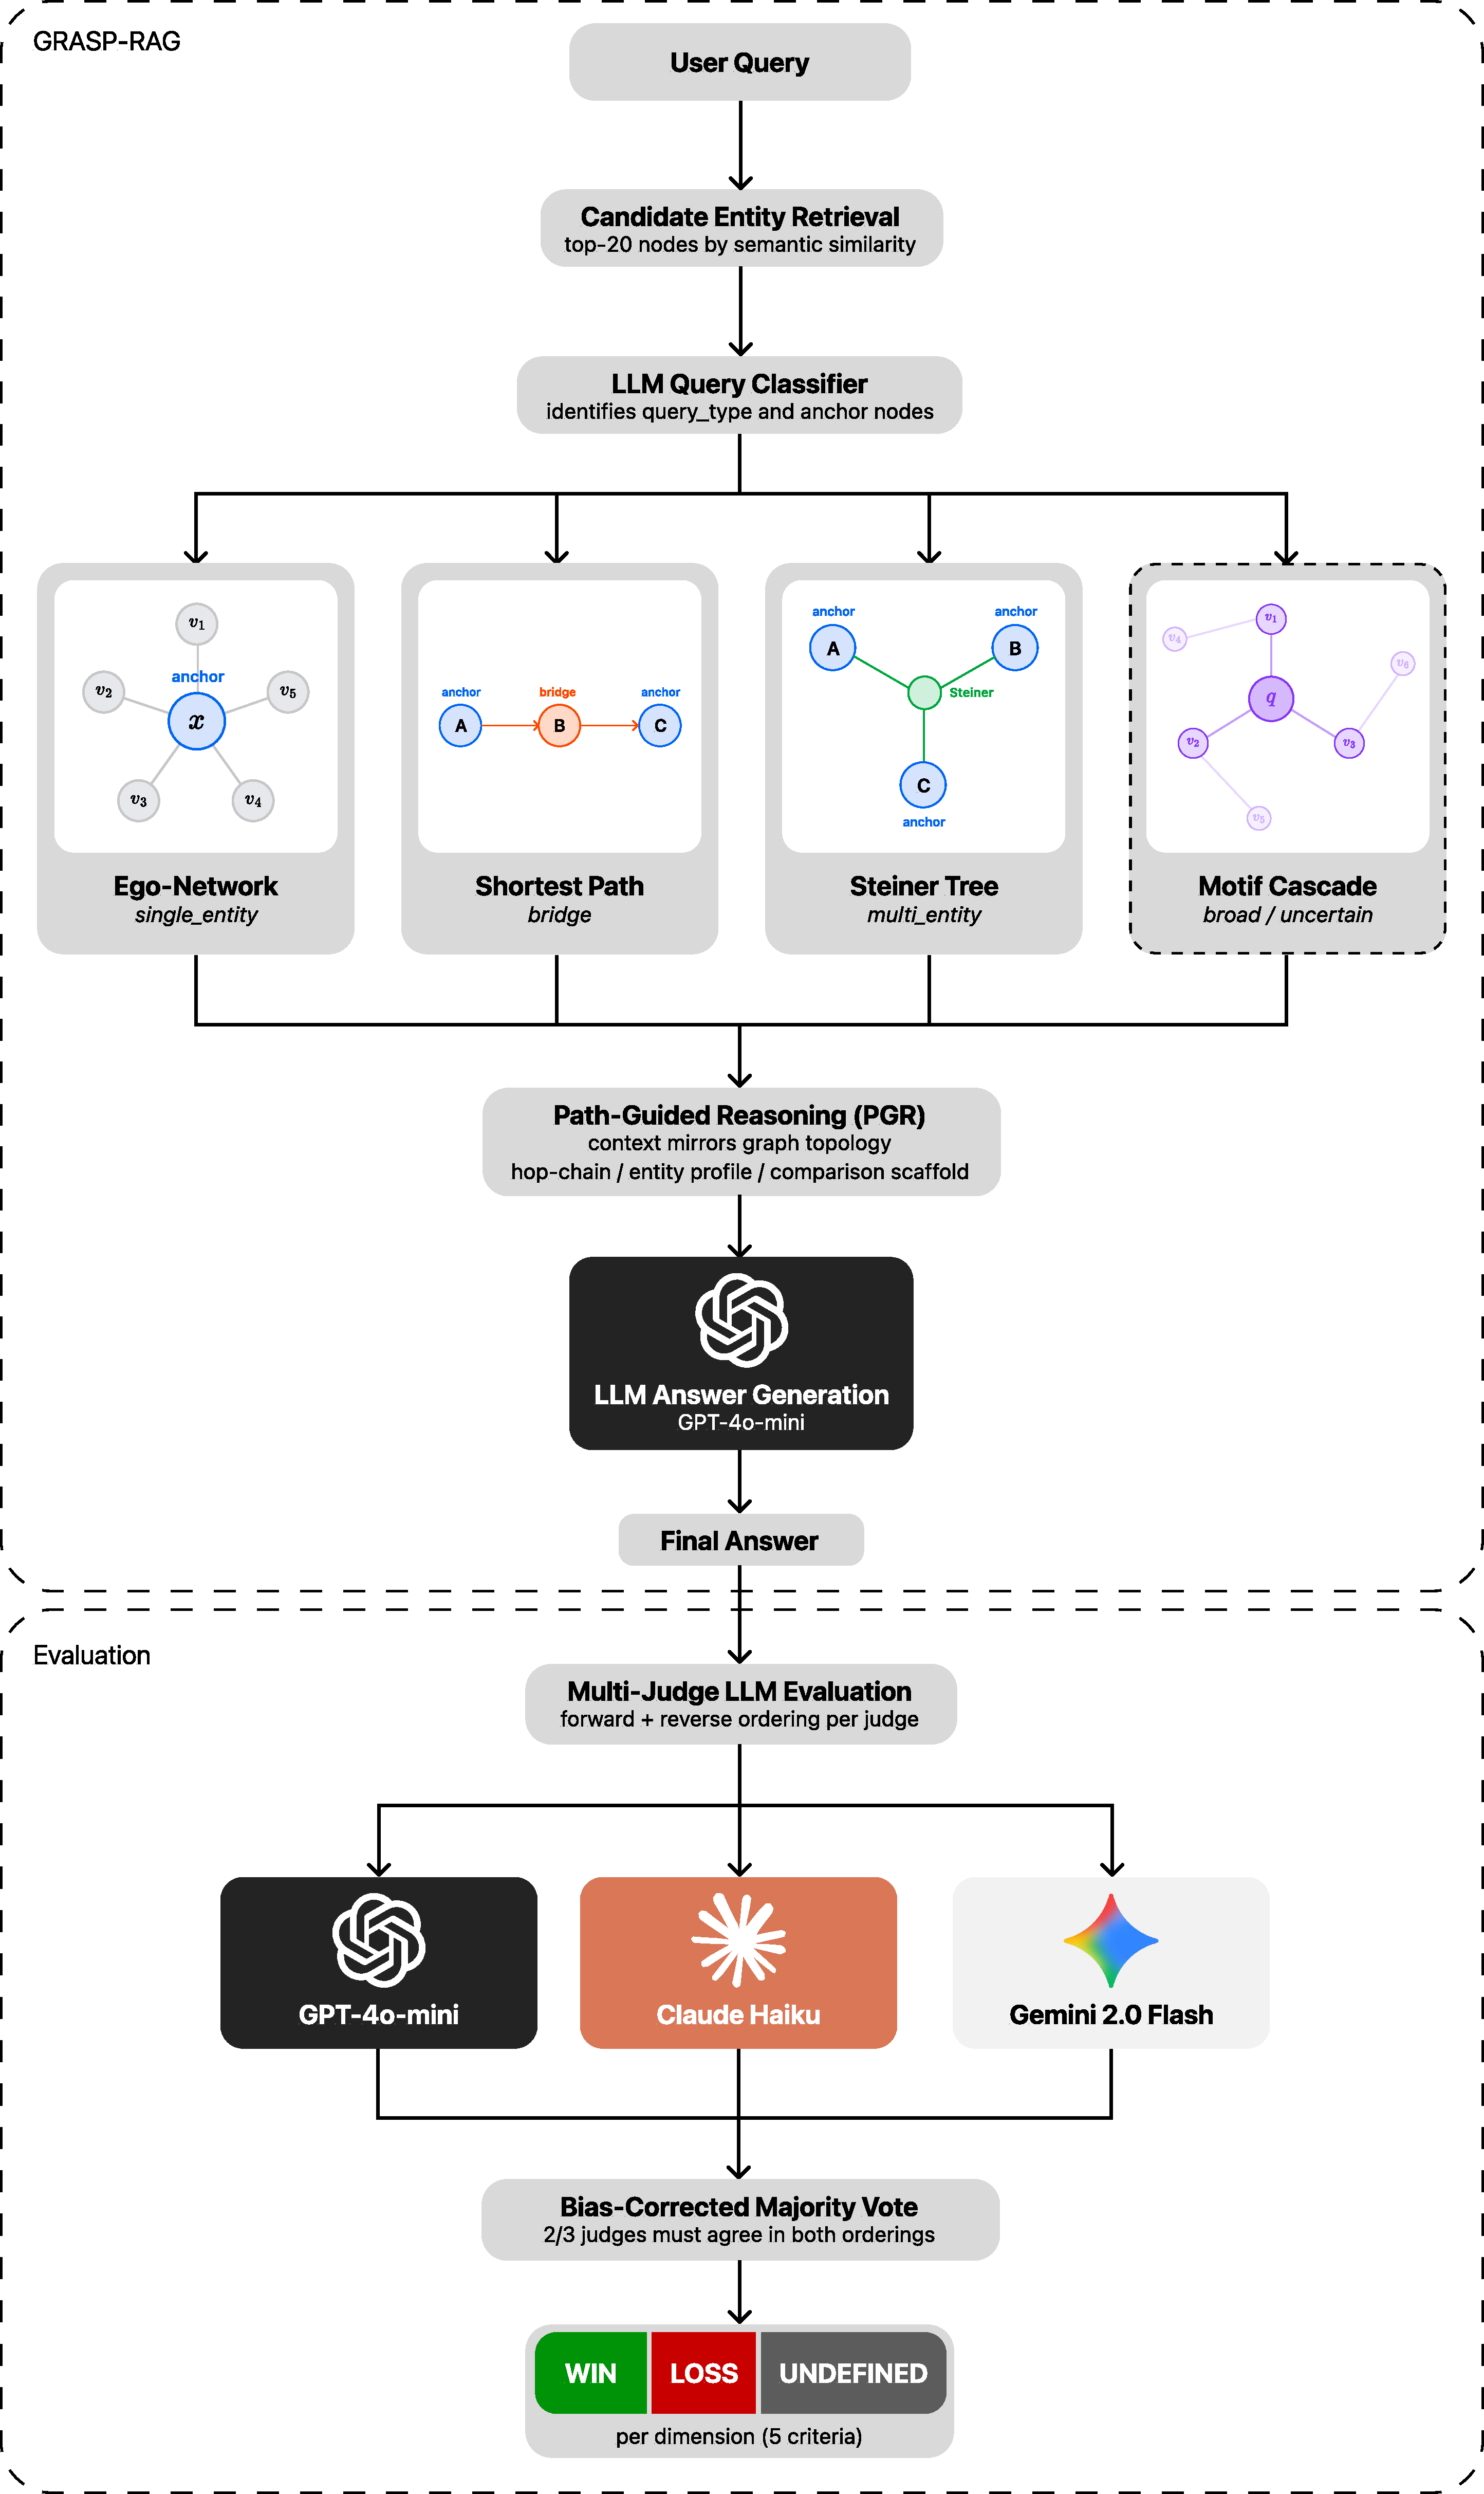
\includegraphics[width=\columnwidth]{system.pdf}
  \caption{GRASP-RAG system overview. \textbf{Top (pipeline):} a user query
    passes through candidate entity retrieval, an LLM classifier, one of four
    motif-specific graph algorithms (Ego-Network, Shortest Path, Steiner Tree,
    or hybrid fallback), and topology-aware context structuring before answer
    generation. \textbf{Bottom (evaluation):} three independent LLM judges
    (GPT-4o-mini, Claude Haiku, Gemini~2.0~Flash) each run forward and reversed
    orderings; a bias-corrected majority vote yields Win, Loss, or Undefined
    per dimension.}
  \label{fig:system}
\end{figure}

\subsection{Query Types and Retrieval Motifs}
\label{sec:motifs_table}

Table~\ref{tab:motifs} defines the four query types and their retrieval motifs,
and Figure~\ref{fig:motifs} illustrates the subgraph shape each one produces.
Each row maps a linguistic question shape to the graph algorithm whose subgraph
structure best matches the answer that shape requires.

\begin{table*}[t]
\caption{GRASP-RAG query types, retrieval motifs, prior-work inspiration, and
  example questions. The classifier routes each query to the matching motif at
  inference time. LightRAG hybrid also serves as the confidence-score fallback
  for any query type when $c(\mathcal{S}) < 0.04$; see
  \S\ref{sec:motif} (Confidence and fallback).}
\label{tab:motifs}
\centering
\renewcommand{\arraystretch}{1.25}
\setlength{\tabcolsep}{4pt}
\begin{tabular}{llp{2.6cm}p{3.6cm}p{5.0cm}}
\toprule
\textbf{Query Type} & \textbf{Motif} & \textbf{Algorithm} &
  \textbf{Inspired by} & \textbf{Example Question} \\
\midrule
Single-entity & Ego-network &
  1-hop neighborhood expansion from anchor node &
  LightRAG local mode~\cite{guo2024lightrag} &
  \textit{``What is the Netfilter Subsystem?''} \\
Bridge & Bidirectional shortest path &
  Shortest path + simple paths of at most 3 hops between two anchor nodes &
  PathRAG relational paths~\cite{chen2025pathrag} &
  \textit{``What connects Rational Grazing to Polyface Farm?''} \\
Multi-entity & Steiner tree &
  Kou et al.\ approximation spanning all anchors~\cite{kou1981fast} &
  G-Retriever prize-collecting Steiner tree~\cite{he2024g} &
  \textit{``How do Varroa Mite, Colony Collapse Disorder, and Neonicotinoids interact?''} \\
Broad & LightRAG hybrid &
  Vector-similarity chunk retrieval combined with keyword graph traversal &
  LightRAG hybrid mode~\cite{guo2024lightrag} &
  \textit{``What are the major sustainability themes across modern farming?''} \\
\bottomrule
\end{tabular}
\end{table*}

\subsection{Problem Formulation}
Let $\mathcal{G} = (\mathcal{V}, \mathcal{E})$ be a knowledge graph where each
node $v$ carries (type, description, source chunk IDs) and each edge $(u,v)$
carries (keywords, weight $w \in \mathbb{R}^+$).
We treat $\mathcal{G}$ as undirected for all path and tree computations.
$\mathcal{N}(v) = \{u \in \mathcal{V} : (v,u)\in\mathcal{E}\ \text{or}\ (u,v)\in\mathcal{E}\}$
denotes the neighbor set of node $v$.
Given query $q$, the goal is to retrieve a subgraph
$\mathcal{S} = (\mathcal{V}_\mathcal{S}, \mathcal{E}_\mathcal{S}) \subseteq \mathcal{G}$
and generate an accurate, grounded answer.

\subsection{Query Classification and Anchor Extraction}
\label{sec:classify}

Given $q$, GRASP-RAG infers query type $\tau$ and anchor nodes $\mathcal{A}$:
\begin{equation*}
  (\tau,\, \mathcal{A}) = \textsc{Classify}(q,\, \mathcal{C})
\end{equation*}
where $\tau \in \{\texttt{single},\, \texttt{bridge},\, \texttt{multi},\,
\texttt{broad}\}$ and $\mathcal{C}$ is a candidate list of up to 20 real graph
node names retrieved \emph{before} the classifier is called.
Candidates are drawn from both the entity VDB and the relationship VDB in
parallel: relationship endpoints surface entity names that the entity VDB alone
may miss, improving anchor recall on queries that phrase entities as relations
(e.g., ``the connection between X and Y'').
The classifier must choose anchors only from $\mathcal{C}$, eliminating
entity-linking errors from name paraphrasing.
If anchor linking fails entirely, the query type is demoted to
\texttt{broad}.

\subsection{Adaptive Motif Selection}
\label{sec:motif}

Based on $(\tau, \mathcal{A})$, GRASP-RAG selects one of four retrieval motifs.

\paragraph{Motif 1 — Ego-network (\texttt{single}).}
$\mathcal{S} = \mathcal{G}[\{n_1\} \cup \mathcal{N}(n_1)]$, the subgraph of
$\mathcal{G}$ induced by the anchor node and its neighbors.
Sufficient and precise for definitional queries: one entity's immediate
neighborhood carries its type, description, relations, and source passages.

\paragraph{Motif 2 — Bridge path (\texttt{bridge}).}
$\mathcal{S}$ is the union of the shortest path between anchor nodes $n_1$ and
$n_2$ and all simple paths of at most 3 hops between them.
Candidate paths are ranked by edge keyword relevance to the query and the
highest-ranked path is selected as the primary reasoning chain.
If no path exists, ego-networks from both anchors serve as a fallback.

\paragraph{Motif 3 — Steiner tree (\texttt{multi}).}
$\mathcal{S} = \textsc{SteinerTree}(\mathcal{G}, \mathcal{A})$ via the
$2(1-1/k)$-approximation~\cite{kou1981fast}, where $k = |\mathcal{A}|$ is
the number of terminal (anchor) nodes: the minimum connected subgraph
spanning all anchor nodes.
Pairwise shortest paths serve as a fallback if the approximation fails on a
disconnected subgraph.

\paragraph{Motif 4 — Hybrid retrieval (\texttt{broad}).}
Broad queries have no specific entity anchors, so graph-traversal motifs do
not apply.
GRASP-RAG delegates to LightRAG's \texttt{hybrid} mode, which combines
vector-similarity chunk retrieval with keyword-based graph traversal.

\paragraph{Confidence and fallback.}
GRASP-RAG derives a structural confidence score. Let $|\mathcal{E}_\mathcal{S}|$
be the number of \emph{distinct} edges in $\mathcal{S}$ and
$|\mathcal{V}_\mathcal{S}|$ the number of distinct nodes covered.
\begin{equation}
  c(\mathcal{S}) = \begin{cases}
    0 & |\mathcal{V}_\mathcal{S}| \le 1 \\[4pt]
    \dfrac{|\mathcal{E}_\mathcal{S}|}{\dbinom{|\mathcal{V}_\mathcal{S}|}{2}}
      \times \min\left(1,\, \dfrac{\alpha}{|\mathcal{V}_\mathcal{S}|}\right)
    & \text{otherwise}
  \end{cases}
  \label{eq:conf}
\end{equation}
where $\alpha = 8$ is a hyperparameter calibrated on a held-out validation
set. Because $|\mathcal{E}_\mathcal{S}| \le \binom{|\mathcal{V}_\mathcal{S}|}{2}$
for distinct edges, $c(\mathcal{S}) \in [0, 1]$.
When $\tau = \texttt{broad}$ or $c(\mathcal{S}) < 0.04$, GRASP-RAG runs all
three structured motifs in parallel on the top VDB candidates, scores each
resulting context with an LLM verifier (1--5 scale), merges all contexts
scoring $\ge 3.0$, and falls back to LightRAG hybrid if no context scores
above 2.5 (contexts in the interval $[2.5, 3.0)$ are merged only when no
context reaches 3.0).

\subsection{Topology-Aware Context Structuring}
\label{sec:pgr}

Most graph-RAG systems serialize retrieved subgraphs as a flat list of passages
or triples regardless of query type.
GRASP-RAG instead structures each motif's output to mirror the answer's
topology.

\paragraph{Bridge context.}
For a retrieved path $[v_0, v_1, \ldots, v_k]$, the context alternates entity
nodes labeled \texttt{[Step $i$ --- Entity: $v$]} with edge descriptions
labeled \texttt{[Step $j$ --- Connection: $v_i \to v_{i+1}$]}.
This labeling makes it harder for the LLM to skip the intermediate (bridge)
entity when generating an answer, though we have not measured inclusion rates
experimentally.

\paragraph{Single-entity context.}
The anchor's description, type, direct connections, and source passages are
assembled into a structured entity profile.

\paragraph{Multi-entity context.}
Per-entity profiles are followed by an explicit connection map between entities.

A single shared generation prompt is used across all motifs; the motif-specific
structure lives entirely in the context, not in the prompt instruction.

% ── Motifs figure (single-column) ────────────────────────────────────────────
\begin{figure}[t]
  \centering
  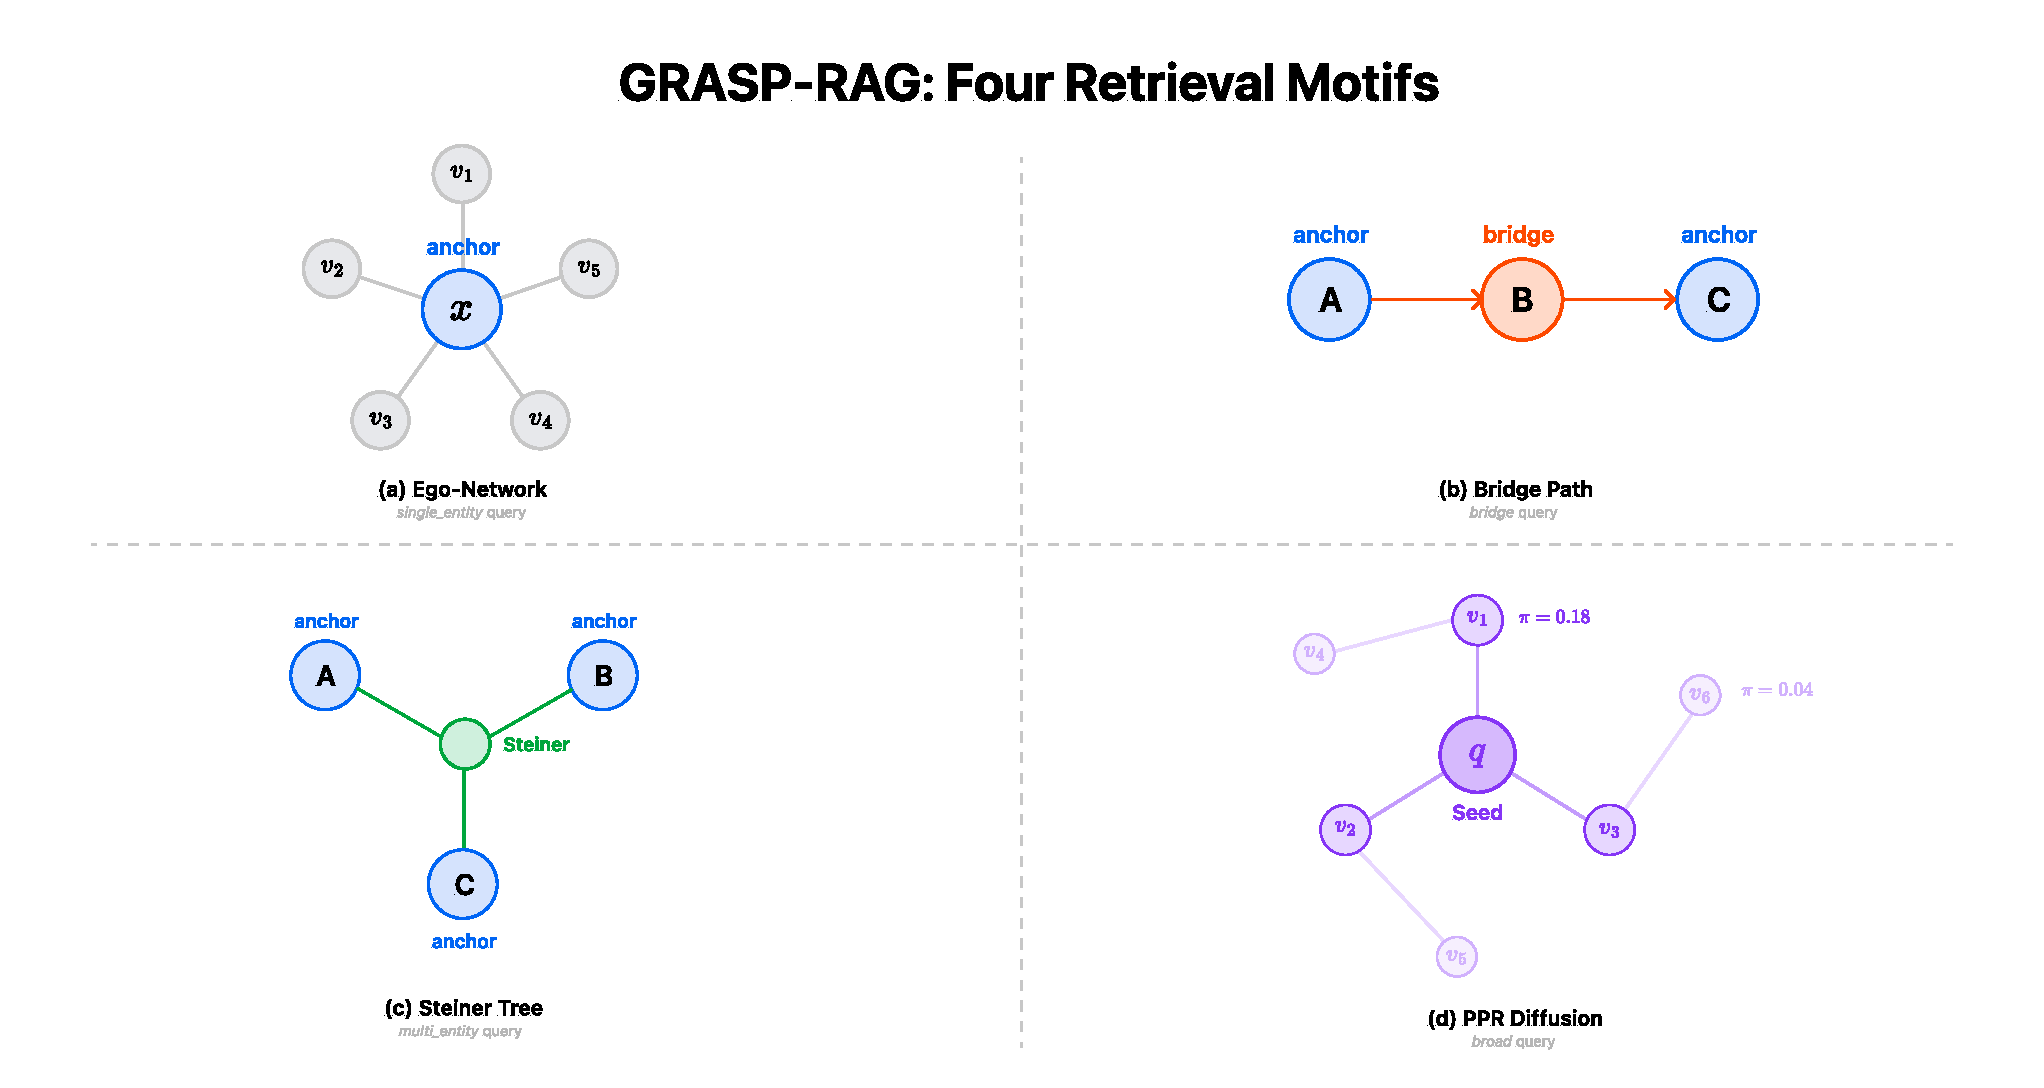
\includegraphics[width=\columnwidth]{fig_motifs.pdf}
  \caption{The four GRASP-RAG retrieval motifs. Blue nodes are query anchors;
    orange is the bridge intermediate entity; green is a Steiner intermediate
    node. Each motif targets the subgraph shape required by the corresponding
    query type; the broad motif delegates to LightRAG hybrid (not shown).}
  \label{fig:motifs}
\end{figure}

% ── 4. Results and Discussion ─────────────────────────────────────────────────
\section{Results and Discussion}
\label{sec:results}

\subsection{Evaluation Protocol}
\label{sec:eval}

We adopt PathRAG's~\cite{chen2025pathrag} five-dimension head-to-head
evaluation criteria extended to a multi-judge protocol.
Each GRASP-RAG answer is compared against a baseline answer by three
independent judges: GPT-4o-mini, Claude Haiku, and Gemini~2.0~Flash.
Each judge runs twice per comparison---\emph{forward} (GRASP-RAG as Answer~1)
and \emph{reversed} (GRASP-RAG as Answer~2)---to control for position bias;
a win is counted only when both orderings agree on the preferred system.
Final outcomes per dimension (Comprehensiveness, Diversity, Logicality,
Coherence, Relevance) are determined by majority vote across the three judges.
When two or more judges mark a dimension as ``Cannot Evaluate'' because both
answers fail to address the question, the dimension is recorded as
\textbf{Undefined} and excluded from the win/loss denominator.
Win rate is the fraction of (question, dimension) pairs where GRASP-RAG wins,
excluding Undefined decisions.

Two limitations of this protocol are worth stating upfront.
GPT-4o-mini serves as both the answer-generation backbone and one of the three
judges; self-preference effects are not independently quantified.
Because all four systems (GRASP-RAG, NaiveRAG, LightRAG, PathRAG) use
GPT-4o-mini for generation, however, self-preference cannot systematically
favour GRASP-RAG over baselines in absolute terms---the concern is rather
that GPT-4o-mini-as-judge may prefer certain answer structures, a confound
the current protocol does not control.
Second, each per-cell result is a point estimate over 100--405 questions, so
numerical differences smaller than a few percentage points should not be
over-interpreted.

\subsection{Experiment 1: Win Rate on UltraDomain}
\label{sec:exp1}

The goal of Experiment~1 is to measure whether GRASP-RAG's answers are
factually closer to expert-written references than baseline answers.
We use the UltraDomain benchmark~\cite{ding2024ultradomain} questions, which
carry reference answers written by domain experts, and evaluate with a
reference-anchored judge that asks which answer is \emph{more accurate relative
to the reference}---not which the judge prefers in isolation.
This is a harder and more externally valid comparison than pairwise preference
without a reference.
UltraDomain's reference answers are provided by the benchmark's creators and
described as domain-expert-authored; we have not independently verified the
credentials of the authors or the factual accuracy of the references.

Table~\ref{tab:winrate} reports GRASP-RAG's win rate against each baseline,
averaged across all five evaluation dimensions.
Questions per domain: 100 (Agriculture), 100 (CS), 405 (Legal), 180 (Health);
differing sample sizes reflect the question sets available per domain and
affect the statistical reliability of per-domain comparisons.
Legal had 426 independently labelled questions in total; 21 lacked evaluation results
and are excluded from win-rate calculations but included in the classifier
confusion matrix (Figure~\ref{fig:confusion}), which accounts for the
difference between the 806-question matrix and the 785-question per-type
Table~\ref{tab:winrate_bytype}.
The Undef.\% column shows the fraction of dimension decisions where both
systems failed simultaneously (vs.\ LightRAG; other baselines are similar).

\begin{table}[t]
\caption{GRASP-RAG win rate (\%) vs.\ each baseline, averaged across all five
  evaluation dimensions. Win rate\,=\,wins\,/\,(wins\,+\,losses) per
  (question\,$\times$\,dimension) pair; Undefined outcomes excluded.
  Baselines: NaiveRAG = dense-passage retrieval; LightRAG = KG hybrid
  retrieval; PathRAG = flow-based path retrieval.
  Bold = highest win rate per data row.
  Undef.\%$^{\dag}$ = fraction of dimension decisions where both systems
  failed simultaneously; $^{\dag}$reported vs.\ LightRAG---rates vs.\
  other baselines are similar.}
\label{tab:winrate}
\centering
\renewcommand{\arraystretch}{1.15}
\setlength{\tabcolsep}{2.8pt}
\begin{tabular}{lrcccr}
\toprule
\textbf{Domain} & \textbf{n} & \textbf{vs NaiveRAG} & \textbf{vs LightRAG} &
  \textbf{vs PathRAG} & \textbf{Undef.\%}$^{\dag}$ \\
\midrule
Agriculture & 100 &          65.2 &          77.7 & \textbf{79.7} & 23.8 \\
CS          & 100 &          83.2 & \textbf{86.3} &          83.7 & 17.0 \\
Legal       & 405 &          39.5 &          52.5 & \textbf{74.2} & 25.1 \\
Health      & 180 &          65.4 &          77.0 & \textbf{81.3} & 28.1 \\
\midrule
\textbf{Average} & --- & 63.3 & 73.4 & \textbf{79.7} & 23.5 \\
\bottomrule
\end{tabular}
\end{table}

The clearest pattern in Table~\ref{tab:winrate} is that GRASP-RAG's most
consistent advantage is against \emph{PathRAG}, the strongest baseline.
The average win rate of 79.7\% against PathRAG holds across all four domains
and is the most stable number in the table; it remains above 74\% in every
domain, reaching a minimum of 74.2\% in Legal where GRASP-RAG struggles
against the other baselines.
Against LightRAG the story is also positive---73.4\% average---though the
Legal result (52.5\%) is close to parity and the Undefined fraction is
substantial everywhere (17--28\%), meaning a significant share of questions
causes both systems to produce uninformative answers.

The Legal domain against NaiveRAG (39.5\%) is the one result where GRASP-RAG
clearly loses, and the cause is two-fold.
Error analysis shows that 53.8\% of losing Legal questions carry a
classifier--reference type mismatch, versus 29.1\% of winning questions: routing
errors concentrate in the loss column.
The most common error is routing a single-entity question through the bridge
path, adding multi-hop traversal where an ego-graph would have been
appropriate.
But misclassification is not the complete explanation.
Oracle bridge questions in Legal (32 questions, classified correctly 84.4\%
of the time) still lose on Relevance at 7.7\% against NaiveRAG.
The Legal KG does not help any graph traversal motif against NaiveRAG's chunk
retrieval.
UltraDomain Legal reference answers emphasise broad coverage of statutory and
regulatory context, and NaiveRAG retrieving many passages from the
KG-extracted content matches that coverage pattern better than a graph
traversal anchored on specific named entities, regardless of which motif is
selected.

\paragraph{On Undefined outcomes.}
The Undefined fraction (17--28\%) is high enough to affect interpretation,
and its distribution across query types is not random.
Broad queries produce Undefined rates 5--18 percentage points above the
per-domain average against NaiveRAG and LightRAG: when both systems fall back
to general keyword or passage retrieval on a thematic question, neither
produces a clearly better answer and judges mark both as unevaluable.
Bridge queries show the opposite pattern against NaiveRAG and LightRAG
(Undefined below average), because GRASP-RAG traverses a specific hop chain
while the baselines do keyword matching---the answers are structurally
different and easy to compare.
Against PathRAG, however, bridge query Undefined rates are above average:
PathRAG's flow-based pruning discards low-frequency edges, so both systems
tend to miss the same specific connections and fail simultaneously.
Undefined fractions are similar across all three baselines (no baseline
systematically avoids shared-failure outcomes), so all three win rates are
comparably affected.

% ── Win-rate bar chart ────────────────────────────────────────────────────────
\begin{figure}[t]
\centering
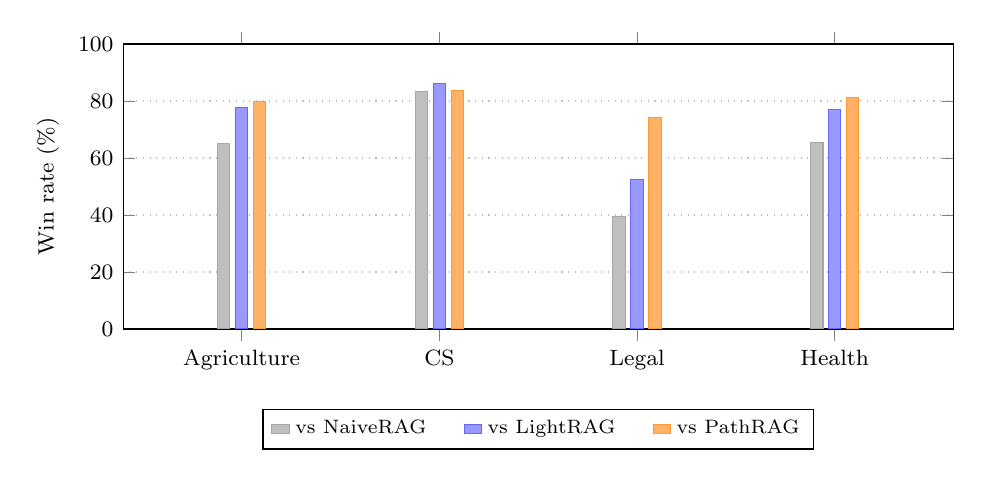
\begin{tikzpicture}
\begin{axis}[
  ybar,
  bar width=4.5pt,
  width=\columnwidth,
  height=5.2cm,
  ymajorgrids=true,
  grid style={dotted,gray!50},
  ylabel={Win rate (\%)},
  ymin=0, ymax=100,
  xtick={0,1,2,3},
  xticklabels={Agriculture, CS, Legal, Health},
  x tick label style={font=\footnotesize},
  y tick label style={font=\footnotesize},
  ylabel style={font=\footnotesize},
  legend style={font=\scriptsize, at={(0.5,-0.28)}, anchor=north,
                legend columns=3, /tikz/every even column/.append style={column sep=0.4cm}},
  legend image code/.code={\draw[#1] (0cm,-0.06cm) rectangle (0.22cm,0.06cm);},
  enlarge x limits=0.2,
]
% vs NaiveRAG
\addplot[fill=gray!50,draw=gray!70] coordinates {(0,65.2)(1,83.2)(2,39.5)(3,65.4)};
% vs LightRAG
\addplot[fill=blue!40,draw=blue!60] coordinates {(0,77.7)(1,86.3)(2,52.5)(3,77.0)};
% vs PathRAG
\addplot[fill=orange!60,draw=orange!80] coordinates {(0,79.7)(1,83.7)(2,74.2)(3,81.3)};
\legend{vs NaiveRAG, vs LightRAG, vs PathRAG}
\end{axis}
\end{tikzpicture}
\caption{GRASP-RAG win rate (\%) by domain and baseline (Experiment~1,
  reference-anchored). The advantage against PathRAG is the most consistent
  across domains; Legal shows a sharp split between baselines.}
\label{fig:winrate_chart}
\end{figure}

\subsection{Experiment 2: Classifier Accuracy and Per-Type Win Rate}
\label{sec:exp2}

Experiment~1 shows that GRASP-RAG wins overall, but it does not tell us
whether the routing machinery is actually working---it is possible the win
comes from the topology-aware context structuring alone, independent of which
motif was selected.
We use two distinct metrics: \emph{classifier accuracy} measures how often the
system's predicted query type matches the independent GPT-4o label; \emph{win
rate} measures how often GRASP-RAG's answer beats a baseline's answer on a
given dimension (regardless of whether the query was correctly typed).
Experiment~2 examines two related questions: how accurately does the
classifier identify query types, and does GRASP-RAG win across types even
when classification is imperfect?

\paragraph{Classifier accuracy.}
We compare GRASP-RAG's automatic type assignments against independently
produced labels from GPT-4o (a stronger labeling model than the GPT-4o-mini
classifier); each label was human-verified by the authors before acceptance.
Figure~\ref{fig:confusion} shows the pooled confusion matrix across all four
domains (806 questions total).
Per-domain overall accuracy ranges from 40.0\% (Agriculture) to 72.0\% (CS),
with Legal and Health at 56.3\% and 50.0\% respectively.

\begin{figure}[t]
  \centering
  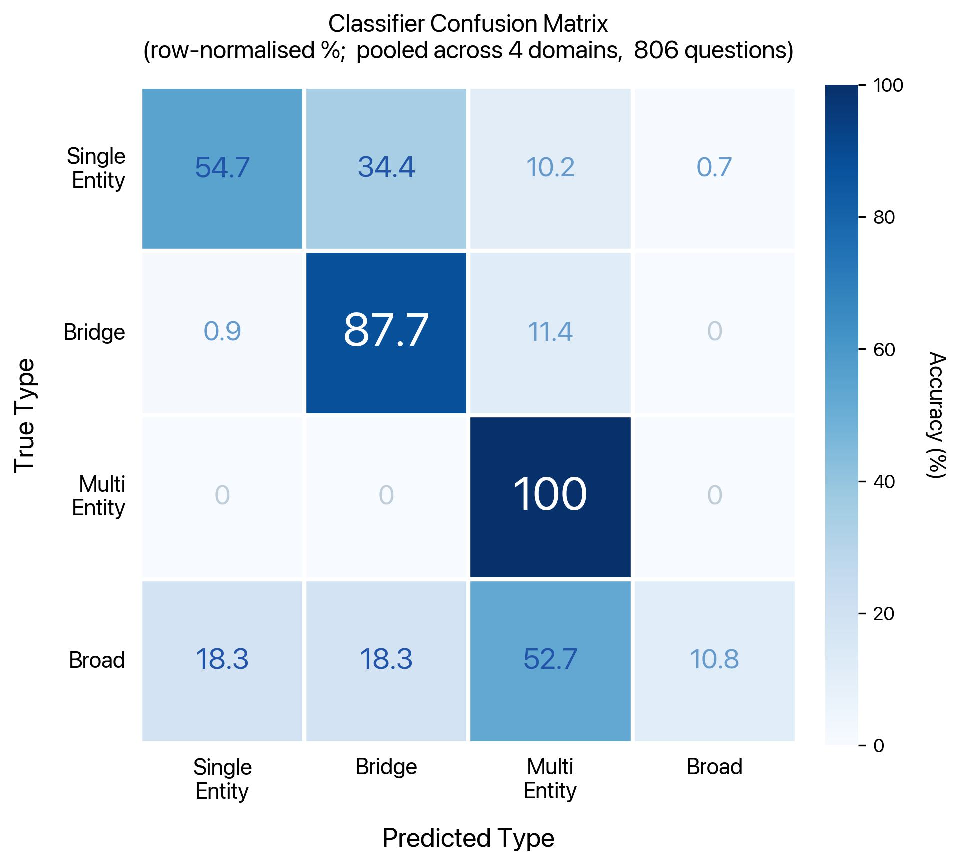
\includegraphics[width=\columnwidth]{confusion_matrix.pdf}
  \caption{Classifier confusion matrix (row-normalised \%), pooled across all
    four UltraDomain domains (806 independently labelled questions, including
    21 Legal questions without evaluation results that are excluded from
    Table~\ref{tab:winrate_bytype}). Bridge is classified reliably
    (87.7\%); broad nearly collapses, with 52.7\% misread as multi-entity.
    Multi-entity shows 100\% on only 9 questions---too small to interpret.}
  \label{fig:confusion}
\end{figure}

Two patterns stand out.
Bridge queries are classified reliably (87.7\% correct pooled): they have
clear structural cues---two named entities and a relational verb.
Broad queries nearly collapse: only 10.8\% are correctly identified, with
52.7\% misread as multi-entity.
This happens because broad questions in the UltraDomain benchmark often
mention domain concepts incidentally, which the classifier interprets as
entity anchors.
Single-entity queries are moderately accurate (54.7\%), with the main
confusion going to bridge (34.4\%)---when a question names a single entity
alongside a domain phrase, the classifier sometimes treats the phrase as a
second anchor.
The multi-entity row shows 100\%, but on only 9 questions across four
domains; that number should not be interpreted as meaningful.

\paragraph{Per-type win rate.}
If classification errors propagate to retrieval errors, we would expect win
rates to drop for the types where the classifier fails.
Table~\ref{tab:winrate_bytype} checks this by grouping Experiment~1's
dimension-level results according to each question's independent label.

\begin{table}[t]
\caption{GRASP-RAG win rate (\%) by independently labeled query type,
  pooled across all four domains (785 evaluated questions; 21 Legal questions
  with independent labels but no evaluation results are excluded; see
  Figure~\ref{fig:confusion} for the full 806-question label set).
  Labels produced by GPT-4o (a stronger labeling model than the GPT-4o-mini
  classifier; each label human-verified by the authors). Win rates stay positive across all types,
  including broad queries where the classifier achieves only 10.8\% accuracy.
  Multi-entity (n\,=\,9) is too small to interpret reliably.}
\label{tab:winrate_bytype}
\centering
\renewcommand{\arraystretch}{1.15}
\setlength{\tabcolsep}{3.5pt}
\begin{tabular}{lcccc}
\toprule
\textbf{Query Type} & \textbf{n} & \textbf{vs NaiveRAG} & \textbf{vs LightRAG} & \textbf{vs PathRAG} \\
\midrule
Single-entity & 569 & 53.4 & 66.2 & 79.9 \\
Bridge        & 114 & 53.6 & 60.1 & 70.9 \\
Multi-entity  & 9   & 60.5 & 72.5 & 74.1 \\
Broad         & 93  & 56.4 & 70.2 & 73.6 \\
\bottomrule
\end{tabular}
\end{table}

The key finding in Table~\ref{tab:winrate_bytype} is that win rates remain
positive for \emph{every} query type against \emph{every} baseline---including
broad queries, where the classifier almost always assigns the wrong label.
This suggests the fallback mechanism limits catastrophic failure when
classification is wrong, though no comparison against a no-fallback baseline
was run to isolate the fallback's independent contribution.
The explanation lies in two mechanisms.
First, when a broad query is misclassified as multi-entity, the Steiner tree
motif runs on the (incorrectly identified) anchor set; the confidence score
\eqref{eq:conf} often falls below the 0.04 threshold on a sparse subgraph,
triggering the fallback to LightRAG hybrid---which is what the broad motif
would have done anyway (we have not logged the fallback trigger rate for
misclassified-broad queries).
Second, even when the wrong motif runs and produces a subgraph, the topology-
aware context structuring may include more specific entity descriptions than a
flat chunk list, which could improve answer quality over baselines that return
generic keyword-matched passages; this has not been isolated experimentally.
This graceful degradation does not make the classification errors
inconsequential---Table~\ref{tab:winrate_bytype} shows that single-entity and
bridge win rates are lower than one would expect from a perfect classifier---
but it does mean the system fails gently rather than catastrophically when
the classifier is wrong.
When grouped by system labels rather than independent labels, win rates follow the
same positive trend across Agriculture, CS, and Health; the exception is
Legal, where questions the classifier routes as bridge achieve only 12--18\%
on Comprehensiveness and Relevance against NaiveRAG, far below the 36--44\%
for questions routed as single-entity.
That bridge-routed group consists predominantly of misclassified single-entity
questions---the dominant classification error in Legal---and matches the
53.8\%-vs-29.1\% mismatch-rate gap described in Section~\ref{sec:exp1}.

\subsection{Discussion}
\label{sec:discussion}

\paragraph{Where the structural advantage is clearest.}
GRASP-RAG's most consistent win is against PathRAG (79.7\% average); one
structural hypothesis is that the motif-routing advantage is most pronounced
against flow-based retrieval.
PathRAG's design assigns reliability scores based on edge traversal frequency:
high-frequency category links (e.g., statute $\to$ provision in Legal,
compound $\to$ metabolic pathway in Health) receive high scores, while
specific bridge edges connecting named entities---which are by definition
low-frequency---may be scored as unreliable and pruned.
GRASP-RAG's bridge motif traverses shortest paths unconditionally, without
filtering by edge frequency.
The Legal domain makes the contrast concrete: GRASP-RAG wins 74.2\% against
PathRAG even while losing to NaiveRAG---a pattern consistent with PathRAG
pruning the low-frequency connections that legal bridge questions target,
though other explanations cannot be ruled out.

\paragraph{Why Legal is hard for everything else.}
Two mechanisms compound in Legal.
Classifier errors concentrate in the loss column: 53.8\% of losing questions
carry a classifier--reference type mismatch, versus 29.1\% of winning questions.
The dominant error is routing a single-entity question through the bridge
path, which introduces extra hops on a question where a direct ego-graph
traversal would have been appropriate.
Domain structure compounds this separately: independently labeled bridge questions in Legal
(correctly classified 84.4\% of the time) still lose on Relevance at 7.7\%
against NaiveRAG.
The Legal KG, built from dense statutory text, is dominated by high-frequency
category links (statute $\to$ provision $\to$ subsection) that connect many
entities but carry little discriminative information per edge.
NaiveRAG retrieving many passages from the same KG-extracted content matches
the broad coverage that Legal reference answers require better than any
graph traversal anchored on named entities.
Improving Legal classification accuracy would reduce losses from misrouted
single-entity questions, but the domain's structural properties mean some gap
against NaiveRAG would likely remain even with perfect routing.

\paragraph{What the per-type pattern tells us.}
Reading Tables~\ref{tab:winrate} and \ref{tab:winrate_bytype} together, the
pattern is: GRASP-RAG outperforms PathRAG most reliably on bridge and single-
entity queries (70.9\% and 79.9\%), and the advantage extends to broad and
multi-entity questions at a lower but still positive level.
The CS domain consistently shows the highest win rates (83--86\% vs.\ all
baselines), which is consistent with CS text having cleaner entity-relation
structure than legal or health text.
Agriculture and Health sit in the middle.
In domains with well-defined entities and explicit relational language, GRASP-
RAG's motif routing gives it a reliable structural advantage; in domains
dominated by procedural or narrative text (Legal), the advantage narrows.

\paragraph{What GRASP-RAG is suited for.}
The results suggest GRASP-RAG is most useful in mixed-question environments
over a structured knowledge graph---that is, applications where a user might
ask definitional, relational, and thematic questions about the same corpus
within the same session.
A fixed-strategy system would do well on the question type it was tuned for
and worse on the others; GRASP-RAG spreads the advantage more evenly by
routing each question to its matched motif.
The classifier's weakness on broad queries (10.8\%) means that corpus-level
thematic questions should ideally be flagged or filtered upstream in a
production system; the per-type win rates show that even on these, the
fallback to LightRAG hybrid is not harmful.

\paragraph{Computational cost.}
GRASP-RAG's cost depends on which execution path is taken.
On the direct path (classifier confident, motif non-broad), each query
requires two GPT-4o-mini calls: one for the classifier and one for answer
generation.
On the cascade path (uncertain classification or broad query type), the
system additionally calls the LLM verifier three times---once per candidate
motif---before generating the answer, for a total of five calls.
NaiveRAG and LightRAG require a single generation call per query; PathRAG is
comparable.
In practice, bridge queries (14\% of the pooled dataset) and correctly
identified single-entity queries (the majority path) take the two-call direct
path; broad queries (12\%) and ambiguous single-entity queries fall through to
cascade or LightRAG hybrid.
The classifier adds one call of latency even on the fast path, which is the
primary cost overhead of the adaptive approach relative to fixed-strategy
baselines.
Latency measurements and per-token cost accounting are left for future
deployment evaluation.

\paragraph{Ablation: context structuring vs.\ graph retrieval.}
To isolate the contribution of topology-aware context serialisation from the
motif's retrieval guarantee, we held routing and graph traversal fixed and
replaced the step-by-step labelled context with a flat serialisation:
entity--description pairs and \texttt{Relation: A\,$\to$\,B | Keywords: \ldots}
triples without hop-chain structure (\textbf{GRASP-RAG-flat}).
Evaluated on Agriculture (100 questions) under the same reference-anchored
multi-judge protocol, the topology-aware variant wins \textbf{62.4\%} of
decided dimension comparisons against GRASP-RAG-flat (Comprehensiveness
62.0\%, Diversity 60.4\%, Logicality 66.0\%, Coherence 63.3\%, Relevance
60.3\%).
The Undefined fraction is high (42--51\%), consistent with both variants
sharing the same retrieval: questions where the retrieved subgraph is
uninformative fail regardless of how context is serialised.
On questions where retrieval provides useful evidence, the step-by-step
topology labels consistently outperform flat serialisation---confirming that
structured context presentation, not just graph traversal, contributes to the
win-rate advantage.

\paragraph{Limitations.}
The context-structuring ablation is evaluated on one domain (Agriculture);
whether the 62.4\% margin replicates on Legal, CS, and Health is left for
future work.
An oracle routing experiment on the same domain---replacing the classifier
with GPT-4o ground-truth labels and VDB-top-$k$ anchor assignment---shows
that GRASP-RAG wins only 42.5\% of decisions against the oracle-routed
variant, meaning perfect routing would recover a further $\sim$15\% of
dimension decisions.
This confirms the classifier is a meaningful bottleneck alongside the
context-structuring contribution.
The anchor assignment in the oracle condition differs from the real system
(VDB candidates vs.\ LLM-extracted named entities), so the gap may partly
reflect anchor quality rather than routing type alone.
Per-judge analysis reveals that GPT-4o-mini, which also generates GRASP-RAG's
answers, awards GRASP-RAG 15--29 percentage points higher win rates against
NaiveRAG and LightRAG than Claude Haiku and Gemini Flash do independently;
the PathRAG comparisons show no such divergence (all three judges agree
within 10\%).
This self-preference inflates the reported NaiveRAG and LightRAG win rates
and means the PathRAG comparison (79.7\% average) is the most credible
result in this evaluation.
The cascade mechanism does not improve substantially over a direct LightRAG
hybrid fallback in the tested settings; we address this in Future Work.

% ── 5. Conclusion and Future Work ─────────────────────────────────────────────
\section{Conclusion and Future Work}

We presented GRASP-RAG, a graph-based RAG system built around a single
observation: the linguistic form of a query already encodes the answer's
graph topology, and retrieval should match that topology rather than ignore
it.
A lightweight classifier routes each query to one of four motifs---ego-network,
shortest-path, Steiner tree, or LightRAG hybrid---and each motif structures
its retrieved subgraph into a topology-aware context that presents the
evidence in the shape the question requires.

Evaluated on four UltraDomain domains with reference-anchored multi-judge
evaluation, GRASP-RAG achieves an average 73.4\% win rate against LightRAG
and 79.7\% against PathRAG.
The advantage against PathRAG is the most consistent, holding above 74\%
in every domain including Legal, where PathRAG's flow-based pruning discards
the low-frequency edges that bridge and relational-chain questions ask about.
Classifier accuracy is moderate overall (40--72\% by domain), with bridge
queries classified reliably (87.7\% pooled) and broad queries nearly failing
(10.8\%), yet per-type win rates stay positive everywhere because the
confidence-based fallback prevents catastrophic misroutes.

Three directions remain open.
First, the broad-query classification problem---where 52.7\% of correctly
broad questions are misread as multi-entity---is the system's clearest
weakness and the most tractable target for improvement.
A classifier that explicitly represents the \emph{absence} of specific entity
anchors, rather than detecting their presence, may handle broad queries better.
Second, the contribution of topology-aware context structuring has not been
isolated from the motif's retrieval guarantee; an ablation running bridge
motif retrieval with flat versus step-by-step context would determine how much
of the win-rate advantage comes from \emph{what} is retrieved versus \emph{how}
it is presented.
Third, the cascade fallback---running all three structured motifs in parallel
when confidence is low---has not been isolated as an independent variable in
the current evaluation; an ablation comparing cascade-on versus a single
direct fallback to LightRAG hybrid is needed to determine whether the added
calls are worth their cost.


% ── References ────────────────────────────────────────────────────────────────
\bibliographystyle{IEEEtran}
\bibliography{references}

\end{document}
